\chapter{Introducción}
\label{cap:capitulo1}
\setcounter{page}{1}

\begin{flushright}
\begin{minipage}[]{10cm}
\emph{La creatividad es la inteligencia divirtiéndose}\\
\end{minipage}\\

Albert Eintein\\
%Autor, \textit{Título}\\
\end{flushright}

\vspace{1cm}

La robótica móvil ha emergido como un campo multidisciplinario que fusiona la
ingeniería, la inteligencia artificial y múltiples ramas de la robótica y la
mecatrónica para crear sistemas capaces de moverse y operar en entornos
dinámicos, interactuando con los mismos de manera que reciben información
mediante sensores y aplican cambios en el medio gracias a sus actuadores, todo
ello manera inteligente debido al software integrado y a su capacidad de
cómputo.
Desde sus inicios, ha sido impulsada por avances significativos en tecnología,
incluyendo sensores y actuadores cada vez más sofisticados, poder de
procesamiento mejorado y algoritmos de control más eficientes.
Estos avances han permitido la aplicación de robots móviles en una amplia gama
de áreas, desde la exploración espacial y submarina hasta la logística
industrial y la atención médica, siendo ya parte indispensable de nuestras vidas
y mejorando la calidad de vida de las personas. En este contexto, la
investigación en robótica móvil se centra en desarrollar sistemas autónomos
capaces de navegar de manera segura y eficiente en entornos desconocidos,
adaptarse a cambios imprevistos y realizar tareas complejas de manera autónoma.
Un buen ejemplo de este tipo de robots se puede ver en la Figura
\ref{fig:rover}, en la que aparecen dos robots enviados a Marte por la NASA en
2020.

\begin{figure} [h!]
  \begin{center}
    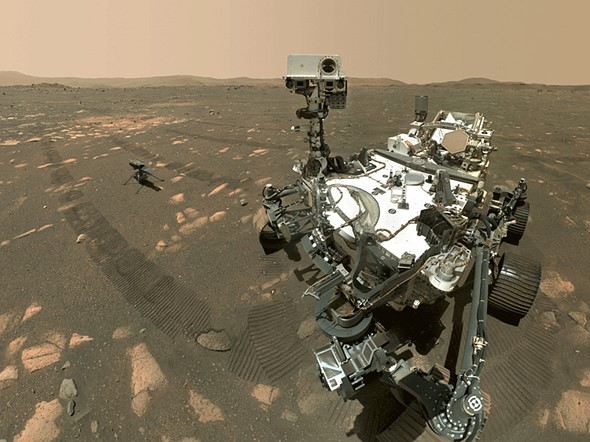
\includegraphics[width=8cm]{figs/perseverance_and_ingenuity_mars_rover_selfie}
  \end{center}
  \caption{Rover Perseverance en Marte con helicoptero Ingenuity de la NASA.}
  \label{fig:rover}
\end{figure}\

La robótica de bajo coste se refiere al desarrollo y la implementación de
sistemas robóticos como los descritos anteriormente utilizando componentes y
recursos económicos, con el objetivo de hacer la tecnología robótica más
accesible y asequible para una amplia gama de aplicaciones y cualquier tipo de
usuario.
Este enfoque busca reducir los costos asociados con la construcción y operación
de robots, utilizando materiales económicos, hardware de bajo coste y técnicas
de fabricación eficientes. En el contexto de la robótica móvil, los sistemas de
bajo coste pueden ofrecer soluciones viables para aplicaciones en las que el
presupuesto es limitado o se requiere un despliegue a gran escala.
Estos robots pueden desempeñar un papel crucial en áreas como la educación, la
investigación académica, la asistencia social y la exploración de entornos
remotos o peligrosos.
Además de su utilidad práctica, la robótica de bajo coste también promueve la
innovación y el desarrollo de nuevas tecnologías al proporcionar una plataforma
accesible para la experimentación y la creatividad abierta a una amplia
comunidad.

%[TODO] citar Figura \ref{fig:sora_q}

\begin{figure} [h!]
  \begin{center}
    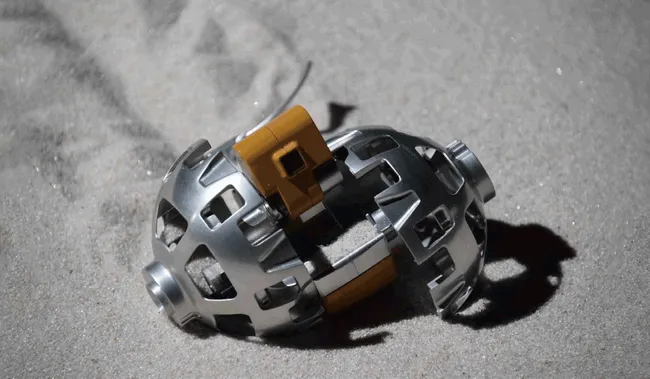
\includegraphics[width=8cm]{figs/SoraQ_lunar_robot_JAXA}
  \end{center}
  \caption{Sora-Q, robot de bajo coste enviado a la Luna, por la JAXA y comercializado por 150€.}
  \label{fig:sora_q}
\end{figure}\

En España, como en el resto de la comunidad europea, el enfoque educativo ha
visto cada vez más claro la relevancia de incluir la robótica en los programas
educativos, ya que es un instrumento valioso para promover la creatividad, el
pensamiento crítico y las habilidades tecnológicas de los alumnos.
En las escuelas primarias y secundarias, se ha visto un incremento en los
últimos años en la implementación de programas educativos que incluyen
actividades prácticas de robótica. Los estudiantes no solo aprenden conceptos
básicos de programación y robótica, sino que también aprenden a trabajar en
equipo y a resolver problemas complejos.
Además, la robótica educativa se ha convertido en un recurso valioso para
aumentar la participación y el interés de los estudiantes en los campos STEM,
preparándolos para futuras carreras relacionadas con la tecnología.

%[TODO] añadir y citar Figura \ref{fig:arduino}

\begin{figure} [h!]
  \begin{center}
    \includegraphics[width=8cm]{figs/Arduino}
  \end{center}
  \caption{Arduino.}
  \label{fig:arduino}
\end{figure}\

Dicha educación robótica suele basarse en la robótica móvil, esto se debe al
hecho de que ver el resultado en movimiento genera en los estudiantes una
sensación de motivación, ilusión por aprender y una realización satisfactoria,
lo cual ayuda en gran medida al su aprendizaje.
También suele basarse en robotica de bajo coste, debido a la baja capacidad de
adquisición de los centros, por su gran numero de alumnos, a los que no podrían
proveer de sistemas de este calibre de otra manera.
Comúnmente se utilizan placas como Arduino o similares, que resultan ideales
para propósitos educativos, sin embargo, estas plataformas también imponen
ciertas limitaciones en la capacidad del robot y en la posibilidad de añadir
hardware periférico más complejo, y por tanto en la propia creatividad y
aprendizaje de los estudiantes, restringiendo así su capacidad y potencial de
creación.
A medida que sus conocimientos avanzan, muchos estudiantes se enfrentan al
desafío de dar el siguiente paso: la programación de robots con ROS, la
plataforma estándar por excelencia, que presenta un considerable escalón de
aprendizaje, ya que para su correcto uso no solo se debe aprender a programar
en un lenguaje complejo, sino que también se debe aprender el entorno que rodea
a este \textit{middleware} robótico, conformado por las telecomunicaciones, la
arquitectura software, la programación modular u orientada a objetos, algoritmos
y estructuras de datos, y un largo etcétera, que suele conllevar decenas de
asignaturas individuales en cualquier grado de robótica en una universidad.
Por lo tanto, resulta evidente la necesidad de un paso intermedio que pueda
servir como puente entre estos dos niveles de aprendizaje, como podría ser el
caso del bachillerato tecnológico en centros de educación secundaria.
Este nivel intermedio facilitaría la transición entre las habilidades adquiridas
en la educación secundaria y los requisitos más avanzados de la universidad en
el campo de la robótica.

%[Párrafo sobre multirobotica].
La multirobotica es un campo de investigación y desarrollo que estudia y
desarrolla sistemas robóticos compuestos por múltiples robots que trabajan
juntos para realizar tareas complejas.
Estos sistemas pueden realizar una variedad de tareas, incluida la exploración
de entornos desconocidos y la búsqueda y rescate en áreas de difícil acceso.
Al aprovechar la capacidad de múltiples robots para trabajar en conjunto y
complementarse entre sí, la multirobotica tiene como objetivo mejorar la
eficiencia y la robustez de los sistemas robóticos.
En esta disciplina se analizan los principios fundamentales, los problemas
técnicos y las aplicaciones prácticas de la multirobotica en varios contextos.

%[Párrafo sobre multirobotica en educación].
En el ámbito educativo, la multirobotica ofrece una oportunidad única para
involucrar a los estudiantes en actividades prácticas y colaborativas.
Al trabajar con sistemas multirobot, los estudiantes no solo adquieren
conocimientos sobre programación, control y mecánica de robots, sino que también
exploran conceptos comoson las telecomunicaciones entre robots, la coordinación,
la planificación y asignación de tareas, la localización y navegación conjunta y
así como la seguridad que se requiere para evitar colisiones entre ellos.
Además, la multirobotica proporciona un entorno de aprendizaje dinámico y
estimulante que despierta aún más la curiosidad y la creatividad de los
estudiantes, preparándolos para enfrentar los desafíos del mundo tecnológico en
constante evolución.

%[Párrafo sobre las telecomunicaciones entre robots]
Las mencionadas telecomunicaciones entre robots son fundamentales en la
multirobotica, ya que garantizan una comunicación rápida, optima,
eficiente y ordenada entre los distintos dispositivos, permitiendo de esta
manera un correcto desempeño de la funcionalidad en cuestión.
Sin embargo, este proceso puede enfrentarse a desafíos como la congestión de la
red, y la consecuente pérdida de mensajes, que pueden ser críticos para el
correcto funcionamiento de los robots.
Por este motivo es crucial gestionar cuidadosamente la cantidad de robots y
mensajes generados, minimizándolos para optimizar el rendimiento del sistema y
evitando de esta manera un cuello de botella.

%[Párrafo sobre flujos de datos y comportamiento reactivo mas simple para educación]
Mantener un flujo de datos correcto es fundamental para solventar los problemas
de telecomunicaciones mencionados en el desarrollo de sistemas de multirobotica.
Además, simplifica el desarrollo del software al proporcionar una clara visión
de la dirección, el origen y el destino de los datos en cada momento.
Esto permite dividir el programa en partes claramente diferenciadas, normalmente
llamadas nodos, modularizándolo y dando lugar a la división del problema último
en varios problemas más simples y fáciles de atajar.
Como resultado, el desarrollo se vuelve un proceso más sostenible y escalable, y
por tanto, más fácil de llevar a cabo por los estudiantes.

%La educación en robótica se basa en la robótica de bajo coste, normalmente en
%placas como Arduino o similares, las cuales son ideales para este uso, y a su
%vez limitan la capacidad del robot en cuestión y el hardware que se puede usar y
%consecuentemente limitan la creatividad y el aprendizaje de los niños. Una vez
%se llega a un cierto nivel de conocimientos, el siguiente paso suele ser la
%programación de robots con ROS2, donde existe un gran escalon de aprendizaje.
%Este trabajo busca simplificar el desarrollo del software en ROS2 y así reducir
%dicho escalón, para hacer más fácil este desarrollo, dando la posibilidad de
%crear aplicaciones robóticas más complejas para robots más completos y que
%permanecen dentro de la categoría de robots de bajo coste y por tanto siguen
%siendo asequibles para instituciones como colegios o institutos.\\

%Escribe aquí un párrafo explicando brevemente lo que vas a contar en este capítulo. En este primer capítulo, el de introducción, se trata de dar un contexto amplio y atractivo del trabajo. Comienza hablando de un contexto general y acaba hablando del contexto más específico en el que se enmarca el proyecto. Es el capítulo idóneo para incluir todas las referencias bibliográficas que hayan tratado este tema; suponen un fuerte respaldo al trabajo.\\

\section{Problemas de ROS en relación con el aprendizaje}
\label{sec:miseccion} % etiqueta para luego referenciar esta sección

%\section{Problemas de ROS en relación con el aprendizaje}
%\label{sec:miseccion} % etiqueta para luego referenciar esta sección

%ROS es el estándar en robótica para la programación de robots, pero tiene un
%problema y es el gran escalón de aprendizaje que existe cuando se pasa de una
%placa simple como arduino, a robots más complejos con máquinas integradas como
%las placas Raspberry Pi o un ordenador portátil directamente. Esto conlleva a una gran
%diferencia entre la robótica que se enseña en los colegios e institutos a la que
%se ebnseña en universidades, y es debido precisamente a la complejidad de código
%y enseñanza de ROS, para los cuales, se requiere incluso de varias asignaturas.
%Por eso en este trabajo se pretende incorporar un paso intermedio en este gran
%escalón.
%
%La propia naturaleza de este \textit{middleware} robótico nos obliga a programar
%nodos que se ejecutan iterativamente en bucle, sin necesidad de generar una
%topología de red concreta para saber de donde vienen o a donde van los datos, lo
%que puede ser un poco complicado de entender a primera vista para los niños.\\
%
%Además de este problema, existe otro relacionado con la congestión de red: los
%nodos de ROS2 se comunican a través de DDS, un protocolo de comunicaciones que
%genera una gran cantidad de mensajes de \textit{Discovery}, lo que conlleva
%consecuentemente a la generación de congestión de la red, y dificulta de esta
%manera la programacion de aplicaciones multiroboticas, que son un posible
%siguiente paso en la enseñanza de la robotica, para entender las comunicaciones
%entre los distintos robots.\\
%
%Este trabajo prentende solucionar tanto el problema del escalón de aprendizaje,
%suponiendo un paso intermedio en la enseñanza de la robótica, y el problema de
%la congestión de red generala por DDS, suponiendo una posible solución a la
%misma.\\
%
%El problema de la congestión se soluciona usando otro protocolo llamado Zenoh,
%con mejores prestaciones que DDS, y la simplicidad del código de ROS2, se ha
%conseguido gracias al uso de un \textit{framework} llamado Zenoh-Flow, que
%funciona sobre el protocolo mencionado y el cual le da nombre. Este
%\textit{framework} está pensado para la programación de flujos de datos,, por lo
%que hay que definir primero un flujo de datos que luego seguiran los nodos,
%activando su iteración al momento de recibir un dato, generando de esta manera
%un flujo de datos que pasa de nodo a nodo, a diferencia de ROS.\\
%
%La implementación conjunta con ROS es posible gracias a que Zenoh-flow permite
%serializar los datos que se quieren enviar, y existe un bridge que los traduce
%de Zenoh a DDS para que los nodos de ROS2 entiendan dicha información. Es por
%este motivo, que si se serializan los mensajes de la misma manera que se hace
%internamente en ROS2, se pueden seguir utilizando nodos ya implementado en ROS2,
%como puede ser la navegación.\\

%En los textos puedes poner palabras en \textit{cursiva}, para aquellas expresiones
%en sentido \textit{figurado}, palabras como \textit{robota}, que está fuera del
%diccionario castellano, o bien para resaltar palabras de una colección:
%\textit{(a)} es la primera letra del abecedario, \textit{(b)} es la segunda, etc.\\

%Al poner las dos líneas del anterior párrafo, este aparecerá separado del anterior. Si no las pongo, los párrafos aparecerán pegados. Sigue el criterio que consideres más oportuno.

\section{Segunda sección}
\label{sec:segundaseccion}

No olvides incluir imágenes y referenciarlas, como la Figura \ref{fig:roomba}.

\begin{figure} [h!]
  \begin{center}
    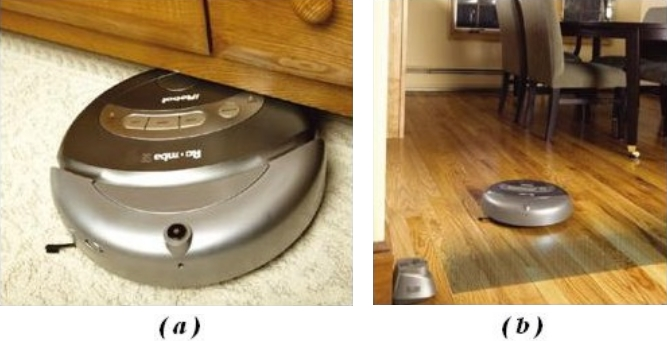
\includegraphics[width=8cm]{figs/roomba}
  \end{center}
  \caption{Robot aspirador Roomba de iRobot.}
  \label{fig:roomba}
\end{figure}\

Ni tampoco olvides de poner las URLs como notas al pie. Por ejemplo, si hablo de la Robocup\footnote{\url{http://www.robocup.org}}.

\subsection{Números}
\label{sec:subseccion}

En lugar de tener secciones interminables, como la Sección \ref{sec:miseccion}, divídelas en subsecciones.

Para hablar de números, mételos en el entorno \textit{math} de \LaTeX, por ejemplo, $1.5Kg$. También puedes usar el símbolo del Euro como aquí: 1.500\euro.

\subsection{Listas}

Cuando describas una colección, usa \texttt{itemize} para ítems o \texttt{enumerate} para enumerados. Por ejemplo:

\begin{itemize}
 \item \textit{Entorno de simulación.} Hemos usado dos entornos de simulación: uno en 3D y otro en 2D.
 \item \textit{Entornos reales.} Dentro del campus, hemos realizado experimentos en Biblioteca y en el edificio de Gestión.
\end{itemize}\

\begin{enumerate}
 \item Primer elemento de la colección.
 \item Segundo elemento de la colección.
\end{enumerate}\

\paragraph{Referencias bibliográficas}
\label{sec:referencias}

Cita, sobre todo en este capítulo, referencias bibliográficas que respalden tu argumento. Para citarlas basta con poner la instrucción \verb|\cite| con el identificador de la cita. Por ejemplo: libros como \cite{vega12e}, artículos como \cite{vega19b}, URLs como \cite{vega19a}, tesis como \cite{vega18b}, congresos como \cite{vega18a}, u otros trabajos fin de grado como \cite{vega08b}.

Las referencias, con todo su contenido, están recogidas en el fichero \texttt{bibliografia.bib}. El contenido de estas referencias está en formato \texttt{BibTex}. Este formato se puede obtener en muchas ocasiones directamente, desde plataformas como \texttt{Google Scholar} u otros repositorios de recursos científicos.

Existen numerosos estilos para reflejar una referencia bibliográfica. El estilo establecido por defecto en este documento es APA, que es uno de los estilos más comunes, pero lo puedes modificar en el archivo \texttt{memoria.tex}; concretamente, cambiando el campo \verb|apalike| a otro en la instrucción \verb|\bibliographystyle{apalike}|. 

\

\

\

Y, para terminar este capítulo, resume brevemente qué vas a contar en los siguientes.
